\documentclass{article}
\usepackage{graphicx}
\usepackage[margin=1.5cm]{geometry}
\usepackage{amsmath}

\begin{document}
\twocolumn

\title{Wednesday Warm Up: Unit 0, Coulomb's Law and E-fields}
\author{Prof. Jordan C. Hanson}

\maketitle

\section{Memory Bank}

\begin{itemize}
\item $\vec{F}_{\rm C} = k q_1 q_2 / r^2 ~~\hat{r}$ ... Coulomb force.
\item $k = 8.988 \times 10^{9}$ N C$^{-2}$ m$^{2}$ ... The constant of proportionality in Coulomb force.
\item $\vec{F} = q\vec{E}$ ... Definition of an electric field.
\item $1e = 1.602 \times 10^{-19}$ Coulombs ... Fundamental unit of charge.
\item $\vec{E} = k q/r^2 ~~\hat{r}$ ... Electric field of a point charge.
\end{itemize}

\section{Electrostatics I: Charges and Fields}

\begin{enumerate}
\item Two small balls, each of mass 5.0 g, are attached to silk threads 50 cm long, which are in turn tied to the same point on the ceiling. When the balls are given the same charge Q, the threads hang at 5.0 degrees to the vertical. What is the magnitude of Q? What are the signs of the two charges? \\ \vspace{4cm}
\item Point charges $q_1 = 2.0$ $\mu$C and $q_2 = 4.0$ $\mu$C are located at $\vec{r}_1 = 4\hat{i} - 2\hat{j} + 5.0\hat{k}$ and $\vec{r}_2 = 8\hat{i} + 5\hat{j} - 9.0\hat{k}$.  (a) What is the magnitude of the force between them? (b) In what direction is the force of $q_2$ on $q_1$? \\ \vspace{4cm}
\item Arrange two point charges $q_1 = -2$ $\mu$C and $q_2 = 4$ $\mu$C along the x-axis so that $\vec{E}=0$ at the origin. \\ \vspace{3cm}
\end{enumerate}

\begin{figure}
\centering
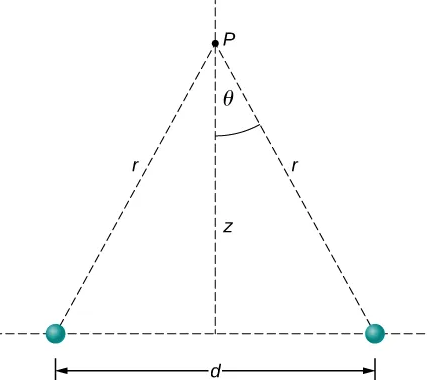
\includegraphics[width=0.33\textwidth]{figures/dipole.png}
\caption{\label{fig:1} Two charges separated by a distance $d$.}
\end{figure}

\section{Electrostatics I: Fields of Charge Distributions}

\begin{enumerate}
\item (a) Consider Fig. \ref{fig:1}.  If the spheres represent positive charges $q$, what is the $\vec{E}$-field at the origin? (b) What is the direction of the $\vec{E}$-field at point $P$?  (c) Derive an expression for the $\vec{E}$-field at point $P$.
\end{enumerate}

\end{document}
